
% \documentclass[draft,11pt]{article}
\chapter{Solving Laplacian
  Linear Equations}

%\allowdisplaybreaks

%%% For this lecture
%\newcommand\symset{S}
%\newcommand\psdset{S_+}
%\newcommand\pdset{S_{++}}

%\newcommand\symsetn{\symset^n}
%\newcommand\psdsetn{\psdset^n}
%\newcommand\pdsetn{\pdset^n}


%\newcommand{\vcliq}[2]{\textsc{Clique}\!\left({#1,#2}\right)}
%\newcommand{\vstar}[2]{\textsc{Star}\!\left({#1,#2}\right)}

%%% added by Hongjie
%\newcommand{\Hongjie}[1]{{\color{red} Hongjie: #1}}
%\newcommand{\vcliqsp}[2]{\textsc{CliqueSample}\!\left({#1,#2}\right)}

%%% layout and code
%\usepackage[vlined, ruled]{algorithm2e}
%\usepackage{float}

%\begin{document}
\sloppy
%\lecture{9 --- Wednesday, April 22nd}
%{Spring 2020}{Rasmus Kyng, Scribe: Hongjie Chen}{Solving Laplacian
%  Linear Equations}

% \todo{introduce stopped martingale}

% \todo{remarks, Tropp and Matrix Freedman and things to know}

% \paragraph{outline}
% \begin{itemize}
% \item objective
% \item precond
% \item algo
% \item martingale
% \item mat conc
% \end{itemize}



\section{Solving Linear Equations Approximately}

Given a Laplacian $\LL$ of a connected graph and a demand vector
$\dd \perp \vecone$, we want to find $\xx^*$ solving the linear equation
$\LL \xx^* = \dd$.
We are going to focus on fast algorithms for finding approximate (but
highly accurate) solutions.

This means we need a notion of an approximate solution.
Since our definition is not special to Laplacians, we state it more
generally for positive semi-definite matrices.
\begin{definition}
  Given PSD matrix $\MM$ and $\dd \in \ker(\MM)^{\perp}$, let
  $\MM \xx^* = \dd$.
  We say that $\xxtil$ is an $\epsilon$-approximate solution to the
  linear equation $\MM \xx = \dd$ if
  \[
    \norm{\xxtil - \xx^*}_{\MM}^2 \leq \epsilon \norm{\xx^*}_{\MM}^2.
  \]
\end{definition}

\begin{remark}
  The requirement $\dd \in \ker(\MM)^{\perp}$ can be removed,
   but this is not important for us.
 \end{remark}

\begin{theorem}[Spielman and Teng (2004) \cite{st04}]
Given a Laplacian $\LL$ of a weighted undirected graph $G = (V,E,\ww)$
with $\abs{E}=m$ and $\abs{V} = n$ and a demand vector $\dd \in \R^V$,
we can find $\xxtil$ that is an $\epsilon$-approximate solution to
$\LL \xx = \dd$, using an algorithm that takes time
$O(m \log^c n \log(1/\epsilon))$ for some fixed constant $c$ and succeeds with probability $1 - 1/n^{10}$.
\end{theorem}
In the original algorithm of Spielman and Teng, the exponent on the
log in the running time was $c \approx 70$.

Today, we are going to see a simpler algorithm. But first, we'll look
at one of the key tools behind all algorithms for solving Laplacian
linear equations quickly.


\section{Preconditioning and
Approximate Gaussian Elimination}
Recall our definition of two positive semi-definite matrices being
approximately equal.
\begin{definition}[Spectral approximation]
  Given $\AA, \BB \in \psdsetn$, we say that
  \[
    \AA \approx_{K} \BB
    \text{ if and only if }
    \frac{1}{1+ K} \AA \preceq \BB \preceq (1+ K) \AA.
    \]
\end{definition}
Suppose we have a positive definite matrix $\MM \in \pdsetn$ and want to
solve a linear equation $\MM \xx =\dd$.
We can do this using gradient descent or accelerated gradient
descent, as we covered in Graded Homework 1.
But if we have access to an easy-to-invert matrix that happens to also
be a good spectral approximation of $\MM$, then we can use this to
speed up the (accelerated) gradient descent algorithm.
An example of this would be that we have a factorization
$\matlow\matlow^{\trp} \approx_{K} \MM$, where $\matlow$ is
lower triangular and sparse, which means we can invert it quickly.

The following lemma, which you will prove in Problem Set 6, makes this
preconditioning precise.
\begin{lemma}
  \label{lem:cholprecond}
  Given a matrix $\MM \in \pdsetn$, a vector $\dd$ and a decomposition $\MM
  \approx_{K} \matlow\matlow^{\trp}$,
  we can find $\xxtil$ that $\epsilon$-approximately solves $\MM \xx =
  \dd$, using
$O( (1+ K)\log(K/\epsilon)(T_{\text{matvec}} + T_{\text{sol}} + n) ) $ time.
\begin{itemize}
\item $T_{\text{matvec}}$ denotes the time required to compute $\MM
  \zz$ given a vector $\zz$, i.e.  a ``matrix-vector multiplication''.
\item  $T_{\text{sol}}$ denotes the time required to compute
  $\matlow^{-1}\zz$ or $(\matlow^{\trp})^{-1}\zz$ given a vector
  $\zz$.
\end{itemize}
\end{lemma}
\paragraph{Dealing with pseudo-inverses.}
When our matrices have a null space, preconditioning becomes slightly
more complicated, but as long as it is easy to project to the
complement of the null space, there's no real issue. The following
describes precisely what we need (but you can ignore the null-space
issue when first reading these notes without losing anything
significant).
\begin{lemma}
  \label{lem:cholprecondpinv}
  Given a matrix $\MM \in \psdsetn$, a vector $\dd \in \ker(\MM)^{\perp}$ and a decomposition $\MM
  \approx_{K} \matlow\calDD\matlow^{\trp}$, where $\matlow$ is invertible,
  we can find $\xxtil$ that $\epsilon$-approximately solves $\MM \xx =
  \dd$, using
${O( (1+ K)\log(K/\epsilon)(T_{\text{matvec}} + T_{\text{sol}} +
T_{\text{proj}} + n) ) }$ time.
\begin{itemize}
\item $T_{\text{matvec}}$ denotes the time required to compute $\MM
  \zz$ given a vector $\zz$, i.e.  a ``matrix-vector multiplication''.
\item  $T_{\text{sol}}$ denotes the time required to compute
  $\matlow^{-1}\zz$ and $(\matlow^{\trp})^{-1}\zz$ and $\calDD^{+}\zz$ given a vector
  $\zz$.
\item $T_{\text{proj}}$ denotes the time required to compute
  $\proj_{\MM} \zz$ given a vector $\zz$.
\end{itemize}
\end{lemma}

\begin{theorem}[Kyng and Sachdeva (2015) \cite{ks16}]
  \label{thm:apxgauss}
Given a Laplacian $\LL$ of a weighted undirected graph $G = (V,E,\ww)$
with $\abs{E}=M$ and $\abs{V} = n$,
we can find a decomposition
$\matlow\matlow^{\trp} \approx_{0.5} \LL $, such that
$\matlow$ has number of non-zeroes $\nnz(\matlow) = O(m \log^3 n)$,
with probability at least $1 - 3/n^{5}$.
in time  $O(m \log^3 n)$.
\end{theorem}
We can combine Theorem~\ref{thm:apxgauss} with
Lemma~\ref{lem:cholprecondpinv} to get a fast algorithm for solving
Laplacian linear equations.
% ...
% \begin{corollary}
%   Given a decomposition $\matlow\matlow^{\trp} \approx_{0.5} \LL $,
% \end{corollary}
\begin{corollary}
  \label{cor:precondsolver}
  Given a Laplacian $\LL$ of a weighted undirected graph $G = (V,E,\ww)$
with $\abs{E}=m$ and $\abs{V} = n$ and a demand vector $\dd \in \R^V$,
we can find $\xxtil$ that is an $\epsilon$-approximate solution to
$\LL \xx = \dd$, using an algorithm that takes time $O(m \log^3 n
\log(1/\epsilon))$ and succeeds with probability $1 - 1/n^{10}$.
\end{corollary}
\begin{proof}[Proof sketch]

  First we need to get a factorization that confirms to
  Lemma~\ref{lem:cholprecondpinv}.
  The decomposition $\matlow\matlow^{\trp}$ provided by
  Theorem~\ref{thm:apxgauss} can be rewritten as
  $\matlow\matlow^{\trp} = \matlowtil \calDD (\matlowtil)^{\trp}$
  where
$\matlowtil$ is equal to $\matlow$ except $\matlow(n,n) = 1$
and we let $\calDD$ be the identity matrix, except $\calDD (n,n)
= 0$.
This ensures $\calDD^{\pinv} = \calDD$ and that $\matlowtil$ is
invertible and lower triagular with  $O(m \log^3 n)$ non-zeros.
We note that the inverse of an invertible lower or upper triangular
  matrix with $N$ non-zeros can be applied in time $O(N)$ given an
  adjacency list representation of the matrix.
  Finally, as $\ker(\matlow\matlow^{\trp}) = \Span\setof{\vecone}$,
we have $\proj_{ \matlowtil \calDD (\matlowtil)^{\trp}}
= \II -\frac{1}{n} \vecone \vecone^{\trp}$, and this projection matrix can be
applied in $O(n)$ time.
Altogether, this means that $T_{\text{matvec}} + T_{\text{sol}} +
T_{\text{proj}} = O(n)$, which suffices to complete the proof.
\end{proof}

\section{Approximate Gaussian Elimination Algorithm}
Recall \emph{Gaussian Elimination / Cholesky decomposition} of a graph Laplacian $\LL$.
We will use $\AA(:,i)$ to denote the the $i$th
column of a matrix $\AA$.
We can write the algorithm as
% \begin{algorithm}[h]
%   \begin{algorithmic}
%  \For{$i = 1$ to $i = n-1$}
%   \State $\ll_i = \frac{1}{\sqrt{\SS_{i-1}(i,i)}} \SS_{i-1}(:,i)$
%   \State  $\SS_{i} = \SS_{i-1} - \ll_i \ll_i^{\trp}.$
%   \EndFor
%   \State $\ll_n = \veczero_{n \times 1}$
%   \State $\matlow=\begin{bmatrix} \ll_1 \cdots \ll_n \end{bmatrix}$
% \end{algorithmic}
% \end{algorithm}

\begin{algorithm}[H]
\label{alg:ge}
\caption{Gaussian Elimination / Cholesky Decomposition}
\KwIn{Graph Laplacian $\LL$}
\KwOut{Lower triangular $\matlow$ s.t. $\matlow\matlow^{\trp} = \LL$}
Let $\SS_0 = \LL$ \;
 \For{$i = 1$ to $i = n-1$}{
$\ll_i = \frac{1}{\sqrt{\SS_{i-1}(i,i)}} \SS_{i-1}(:,i)$\;
$\SS_{i} = \SS_{i-1} - \ll_i \ll_i^{\trp}.$\
}
$\ll_n = \veczero_{n \times 1}$\;
\Return{$\matlow=\begin{bmatrix} \ll_1 \cdots \ll_n \end{bmatrix}$}\;
\end{algorithm}
% Now, for $i = 1$ to $i = n-1$ we define
% \begin{align*}
%   \ll_i &= \frac{1}{\sqrt{\SS_{i-1}(i,i)}} \SS_{i-1}(:,i), \\
%   \SS_{i} &= \SS_{i-1} - \ll_i \ll_i^{\trp}.
% \end{align*}
% Finally, we let $\ll_n = \veczero_{n \times 1}$. It follows that
% $\matlow=\begin{bmatrix} \ll_1 \cdots \ll_n \end{bmatrix}$ is lower
% triangular and $\LL=\matlow\matlow^\trp$.
We want to introduce some notation that will help us describe and
analyze a faster version of Gaussian elimination -- one that uses sampling
to create a sparse approximation of the decomposition.

Consider a Laplacian $\SS$ of a graph $H$ and a vertex $v$ of $H$.
We define $\vstar{v}{\SS}$ to be the Laplacian of the subgraph of $H$
consisting of edges incident on $v$.
We define
\[
\vcliq{v}{\SS} = \vstar{v}{\SS} - \frac{1}{\SS(v,v)} \SS(:,v)  \SS(:,v)^{\trp}
\]
For example, suppose
\[
  \LL =
\left(
\begin{array}{ccc}
W & -\aa^\trp \\
-\aa& \diag(\aa) + \LL_{-1}
\end{array} \right)
\]
Then
\[
\vstar{1}{\LL}
=
\left(
\begin{array}{ccc}
W & -\aa^\trp \\
-\aa& \diag(\aa)
\end{array} \right)
\text{ and }
\vcliq{1}{\LL}
=
\left(
\begin{array}{ccc}
0 &  \veczero \\
\veczero & \diag(\aa) - \frac{1}{W} \aa \aa^\trp
\end{array} \right)
\]
which is illustrated in Figure \ref{fig:schurclique}.
%
\begin{figure}[H]
  \centering
  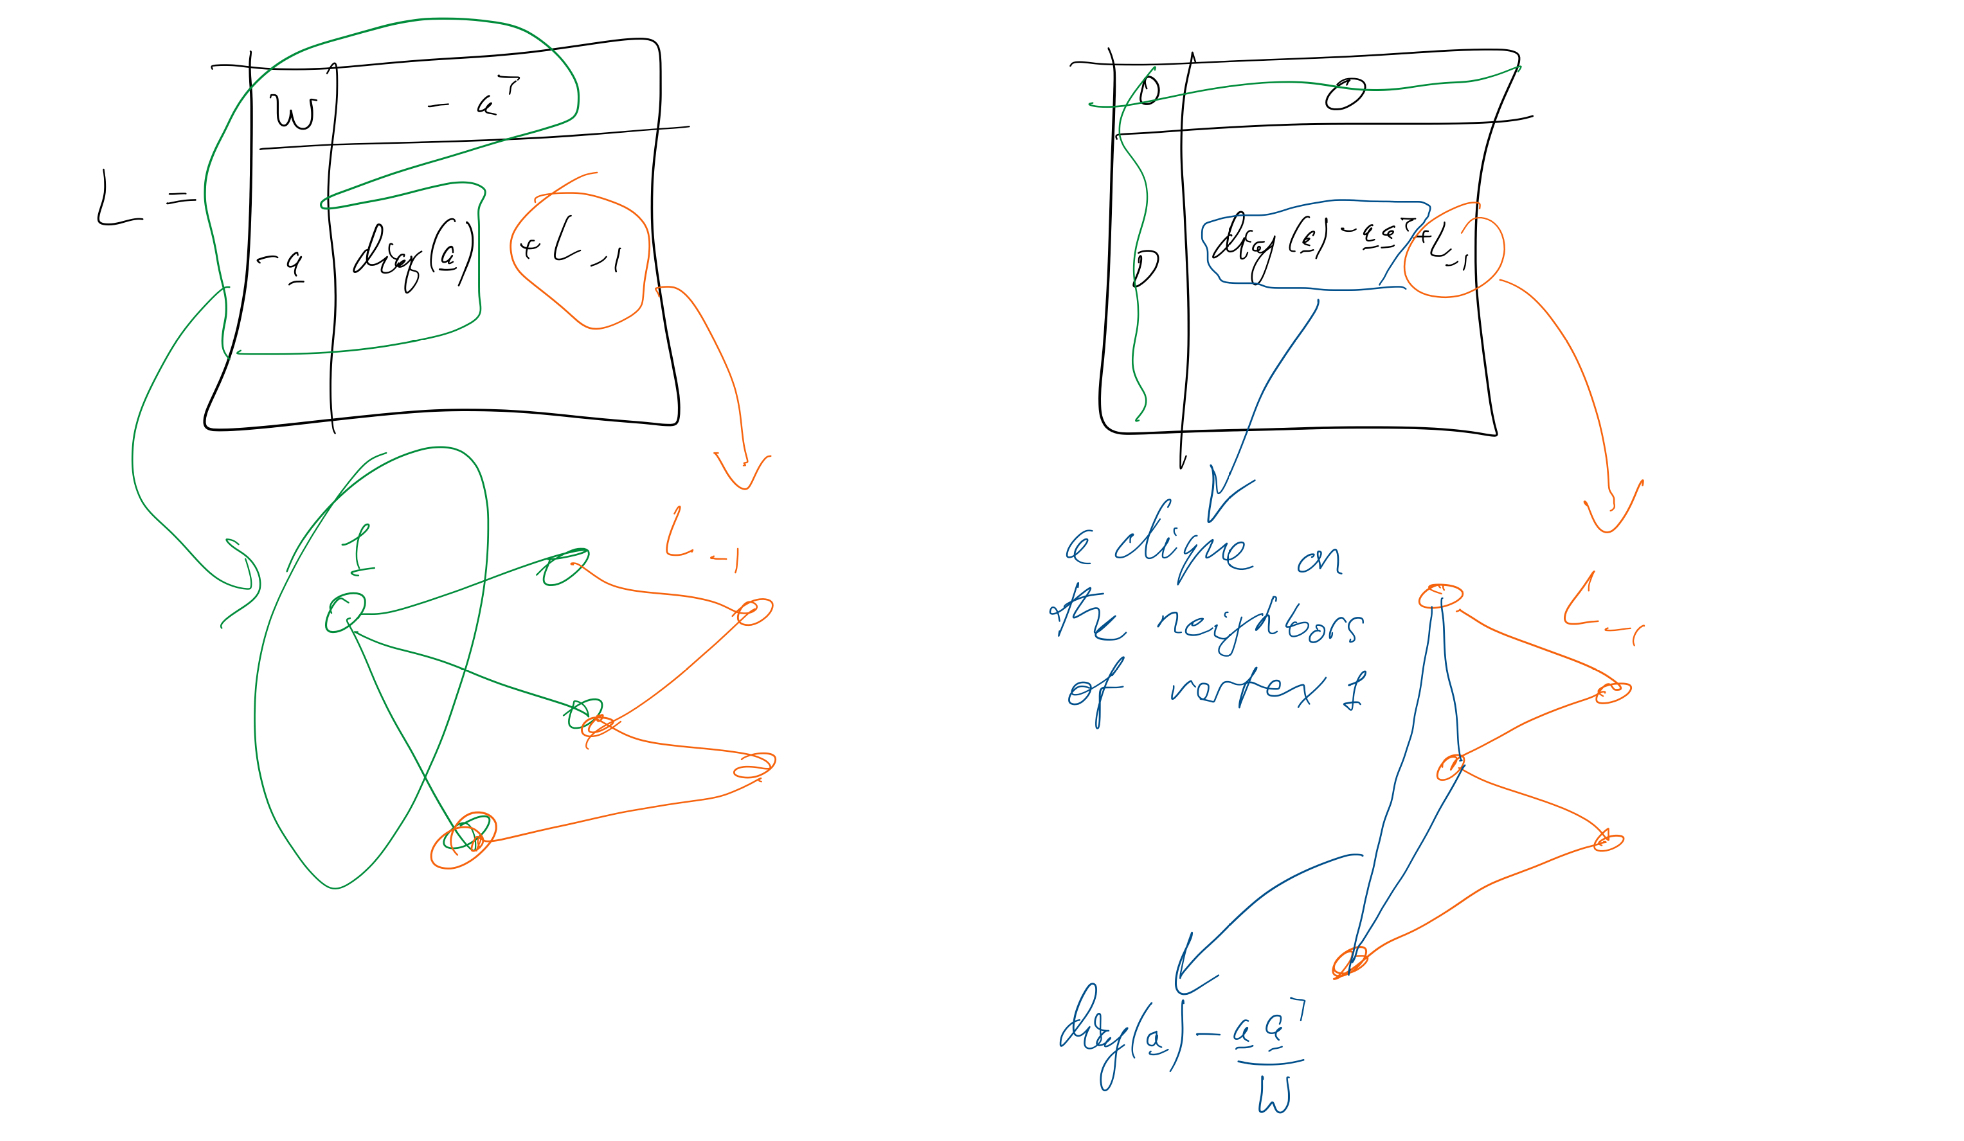
\includegraphics[width=1
  \textwidth]{fig/lecture7_schur-clique.jpeg}
  \caption{Gaussian Elimination:
    $\vcliq{1}{\LL} = \vstar{1}{\LL} - \frac{1}{\LL(1,1)} \LL(:,1)
    \LL(:,1)^{\trp}$.}
      \label{fig:schurclique}
    \end{figure}
In Chapter~\ref{cha:ge}, we proved that $\vcliq{v}{\SS}$ is a graph Laplacian --
it follows from the proof of Claim~\ref{clm:optimgaussclosed} in that lecture.
Thus we have that following.
 \begin{claim}
\label{clm:optimgaussclosedagain}
If $\SS$ is the Laplacian of a connected graph, then
$\vcliq{v}{\SS}$ is a graph Laplacian.
% \begin{enumerate}
% \item $\vcliq{v}{\SS}$ is a graph Laplacian.
% \item
% \end{enumerate}
\end{claim}

Note that in Algorithm~\ref{alg:ge}, we have  $\ll_i\ll_i^\trp = \vstar{v_i}{\SS_{i-1}}-\vcliq{v_i}{\SS_{i-1}}$. The update rule can be rewritten as
\[ \SS_{i} = \SS_{i-1} - \vstar{v_i}{\SS_{i-1}} +
  \vcliq{v_i}{\SS_{i-1}}, \]

This also provides way to understand why
Gaussian Elimination is slow in some cases.
At each step, one vertex is eliminated, but a clique is added to the
subgraph on the remaining vertices, making the graph denser.
And at the $i$th step, computing $\vstar{v_i}{\SS_{i-1}}$
takes around $\deg(v_i)$ time, but computing $\vcliq{v_i}{\SS_{i-1}}$
requires around $\deg(v_i)^2$ time.
In order to speed up Gaussian
Elimination, the algorithmic idea of \cite{ks16}
%\cite{?}
 is to plug in a sparser appproximate of the intended clique instead
 of the entire one.

The following procedure $\vcliqsp{v}{\SS}$ produces a sparse
approximation of $\textsc{clique}(v,\SS)$.
Let $V$ be the vertex set of the graph associated with $\SS$ and $E$
the edge set.
We define $\bb_{i,j} \in \R^V$ to be the vector with
\[
  \bb_{i,j}(i) = 1
  \text{ and }
  \bb_{i,j}(j) = -1
  \text{ and }
  \bb_{i,j}(k) = 0
  \text{ for }
  k \neq i,j.
\]
Given weights $\ww \in \R^E$ and a vertex $v \in V$,
we let
\[
  \ww_v = \sum_{(u,v) \in E} \ww(u,v)
  .
  \]
\begin{algorithm}[H]
\label{alg:cliquesamp}
\caption{$\vcliqsp{v}{\SS}$}
\KwIn{Graph Laplacian $\SS \in \R^{V \times V}$, of a graph with edge
  weights $\ww$, and vertex $v \in V$}
\KwOut{$\YY_v \in \R^{V \times V}$ sparse approximation of
  $\textsc{clique}(v,\SS)$  }
 $\YY_v   \gets  \matzero_{n \times n} $\;
 \ForEach{Multiedge $e
   = (v,i)$ from $v$ to a neighbor $i$}{
    Randomly pick a neighbor $j$ of $v$ with probability $\frac{\ww(j,v)}{\ww_v}$\;
    If $i \neq j$, let $\YY_v   \gets \YY_v + \frac{\ww(i,v)\ww(j,v)}{\ww(i,v)+\ww(j,v)} \bb_{i,j}\bb_{i,j}^\trp$\;
}
\Return{$\YY_v$}\;
\end{algorithm}
% Let $\YY_v = \matzero_{n \times n}$. For each neighbor $i$ of $v$, randomly pick a neighbor $j$ of $v$ with probability $\frac{\ww(j,v)}{\ww_v}$ where $\ww_v = \sum_{u \sim v} \ww(u,v)$ is the sum of weights of edges incident to $v$. If $i\neq j$, then draw an edge with weight $\ww(i,v)\ww(j,v)/(\ww(i,v)+\ww(j,v))$ between $i$ and $j$, i.e. update $\YY_v$ by
% \[ \YY_v \gets \YY_v + \frac{\ww(i,v)\ww(j,v)}{\ww(i,v)+\ww(j,v)} \bb_{i,j}\bb_{i,j}^\trp. \]
%
\begin{remark}
  We can implement each sampling of a neighbor $j$ in $O(1)$ time
  using a classical algorithm known as Walker's method (also known as the Alias
  method or Vose's method).
  This algorithm requires an additional $O(\deg_{\SS}(v))$ time to
  initialize a data structure used for sampling.
  Overall, this means the total time for $O(\deg_{\SS}(v))$ samples is still $O(\deg_{\SS}(v))$.
\end{remark}

% %TODO this paragraph sometimes causes horizontal "badness" failure
% In what sense does $\vcliqsp{v}{\SS}$ produce a sparse approximation
% of the clique $\vcliq{v}{\SS}$ created by Gaussian elimination?
% This is a crucial question, and the next lemma gives part of the
% answer: Namely that the output in expectation equals the clique.
\begin{lemma}\label{lem:cliquesample_expectation}
  $\E{\YY_v} = \vcliq{v}{\SS}$.
\end{lemma}
\begin{proof}
  Let $\CC=\vcliq{v}{\SS}$. Observe that both $\E{\YY_v}$ and $\CC$ are Laplacians. Thus it suffices to verify $\Ex{\YY_v(i,j)}=\CC(i,j)$ for $i\neq j$.
  \[ \CC(i,j) = -\frac{\ww(i,v)\ww(j,v)}{\ww_v}, \]
  \[ \Ex{\YY_v(i,j)} = -\frac{\ww(i,v)\ww(j,v)}{\ww(i,v)+\ww(j,v)} \left( \frac{\ww(j,v)}{\ww_v} + \frac{\ww(i,v)}{\ww_v} \right) = -\frac{\ww(i,v)\ww(j,v)}{\ww_v} = \CC(i,j). \]
\end{proof}
\begin{remark}
  Lemma \ref{lem:cliquesample_expectation} shows that $\vcliqsp{v}{\LL}$ produces the original $\vcliq{v}{\LL}$ in expectation.
\end{remark}

Now, we define \emph{Approximate Gaussian Elimination}.
% Let $\SS_0 = \LL$. Generate a radom permutation $\pi$ on $[n]$. For $i = 1$ to $i = n-1$ we define
% \begin{align*}
%   \ll_i &= \frac{1}{\sqrt{\SS_{i-1}(\pi(i),\pi(i))}} \SS_{i-1}(:,\pi(i)), \\
%   \SS_{i} &= \SS_{i-1} - \vstar{\pi(i)}{\SS_{i-1}} + \vcliqsp{\pi(i)}{\SS_{i-1}}.
              %   \end{align*}

\begin{algorithm}[H]
\label{alg:apxge}
\caption{Approximate Gaussian Elimination / Cholesky Decomposition}
\KwIn{Graph Laplacian $\LL$}
\KwOut{Lower triangular\footnote{$\matlow$ is not actually lower
    triangular. However, if we let $\PP_\pi$ be the permutation matrix
    corresponding to $\pi$, then $\PP_\pi \matlow$ is lower
    triangular. Knowing the ordering that achieves this is enough to
    let us implement forward and backward substitution for solving
    linear equations in $\matlow$ and $\matlow^\trp$.}
  $\matlow$ as
  given in Theorem~\ref{thm:apxgauss}}
Let $\SS_0 = \LL$\;
Generate a random permutation $\pi$ on $[n]$\;
\For{$i = 1$ to $i = n-1$}{
$\ll_i = \frac{1}{\sqrt{\SS_{i-1}(\pi(i),\pi(i))}} \SS_{i-1}(:,\pi(i)) $\;
$\SS_{i} = \SS_{i-1} - \vstar{\pi(i)}{\SS_{i-1}} + \vcliqsp{\pi(i)}{\SS_{i-1}}$\
}
$\ll_n = \veczero_{n \times 1}$\;
\Return{$\matlow=\begin{bmatrix} \ll_1 \cdots \ll_n \end{bmatrix}$ and
$\pi$}\;
\end{algorithm}
% $\PP_\pi$ be the permutation matrix corresponding to $\pi$. It follows that $\matlow =
% \PP_\pi \begin{bmatrix} \ll_1 \cdots \ll_n \end{bmatrix}$ is lower
% triangular and $\LL=\matlow\matlow^\trp$.
Note that if we replace
$\vcliqsp{\pi(i)}{\SS_{i-1}}$ by $\vcliq{\pi(i)}{\SS_{i-1}}$ at each
step, then we can recover Gaussian Elimination, but with a random
elimination order.

\section{Analyzing Approximate Gaussian Elimination}

In this Section, we're going to analyze Approximate Gaussian
Elimination, and see why it works.

Ultimately, the main challenge in proving Theorem~\ref{thm:apxgauss}
will be to prove for the output $\matlow$
of Algorithm~\ref{alg:apxge} that with high probability
\begin{equation}
  \label{eq:relerrgoal}
0.5 \LL
\preceq
\matlow \matlow^{\trp}
\preceq 1.5 \LL
.
\end{equation}
We can reduce this to proving that with high probability
\begin{equation}
\label{eq:spectralnormgoal}
 \norm{\LL^{+/2} (\matlow \matlow^{\trp} -  \LL) \LL^{+/2}} \leq 0.5
\end{equation}
Ultimately, the proof is going to have a lot in common with our proof
of Matrix Bernstein in Lecture 8.
Overall, the lesson there was that when we have a sum of independent,
zero-mean random matrices, we can show that the sum is likely to have
small spectral norm if the spectral norm of each random matrix is
small, and the matrix-valued variance is also small.

Thus, to replicate the proof, we need control over
\begin{enumerate}
\item The \emph{sample norms}.
\item The \emph{sample variance}.

\end{enumerate}

But, there is seemlingly another major obstacle: We are trying to
analyze a process where the samples are far from independent.
Each time we sample edges, we add new edges to the remaining graph,
which we will the later sample again. This creates a lot of
dependencies between the samples, which we have to handle.

However, it turns out that independence is more than what is needed to
prove concentration. Instead, it suffices to have a sequence of random
variables such that each is mean-zero in expectation, conditional on
the previous ones. This is called a martingale difference sequence.
We'll now learn about those.

\subsection{Normalization, a.k.a. Isotropic Position}

Since our analysis requires frequently measuring matrices after right
and left-multiplication by $\LL^{\pinv/2}$, we reintroduce the
``normalizing map'' $\Phi : \R^{n\times n} \to
\R^{n\times n} $
defined by
\[
  \Phi(\AA) = \LL^{\pinv/2}\AA\LL^{\pinv/2}.
  \]
We previously saw this in Lectures 7 and 8.

\subsection{Martingales}

A scalar martingale is a sequence of random variables $Z_0, \ldots,
Z_k$, such that
\begin{align}
\label{eq:martingale}
  \E{Z_i \mid Z_0, \ldots, Z_{i-1}} = Z_{i-1}
.
\end{align}
That is, conditional on the outcome of all the previous random
variables, the expectation of $Z_{i}$ equals $Z_{i-1}$.
If we unravel the sequence of conditional expectations, we
get that \emph{without conditioning}
$\E{Z_k}=\E{Z_0}$.

Typically, we use martingales to show a statement along like  ``$Z_k$
is concentrated around $\E{Z_k}$''.

We can also think of a martingale in terms of the sequence of changes
in the $Z_i$ variables.
Let $X_i = Z_i - Z_{i-1}$.
The sequence of $X_i$s is called a martingale difference sequence.
We can now state the martingale condition as
\[
  \E{X_i \mid Z_0, \ldots, Z_{i-1}} = 0
.
\]
And because $Z_0$ and $X_{1}, \ldots, X_{i-1}$ completely determine
$Z_1,  \ldots, Z_{i-1}$, we could also write
the martingale condition equivalently as
\[
  \E{X_i \mid Z_0, X_1, \ldots, X_{i-1}} = 0
  .
\]
Crucially, we can write
\[
Z_k = Z_0 + \sum_{i=1}^k Z_i - Z_{i-1} = Z_0 + \sum_{i=1}^k X_i
\]
and when we are trying to prove concentration, the martingale difference property
of the $X_i$'s is often ``as good as'' independence, meaning that
$\sum_{i=1}^k X_i$ concentrates similarly to a sum of independent
random variables.




\paragraph{Matrix-valued martingales.}
We can also define matrix-valued martingales.
In this case, we replace the martingalue condition of
Equation~\eqref{eq:martingale}, with the condition that the whole matrix
stays the same in expectation.
For example, we could have a sequence of random matrices $\ZZ_0, \ldots,
\ZZ_k \in \R^{n \times n}$, such that
\begin{align}
\label{eq:matmartingale}
  \E{\ZZ_i \mid \ZZ_0, \ldots, \ZZ_{i-1}} = \ZZ_{i-1}
.
\end{align}
\begin{lemma}\label{lem:ApxGE_martingale}
  Let $\LL_i = \SS_i + \sum_{j=1}^i \ll_j\ll_j^\trp$ for $i=1,...,n$ and $\LL_0=\SS_0=\LL$. Then
  \[ \E{\LL_i | \text{all random variables before } \vcliqsp{\pi(i)}{\SS_{i-1}} } = \LL_{i-1}. \]
\end{lemma}
\begin{proof}
  Let's only consider $i=1$ here as other cases are similar.
  \[ \LL_0 = \LL = \ll_1\ll_1^\trp + \vcliq{v}{\LL} + \LL_{-1} \]
  \begin{align*}
    \LL_1 &= \ll_1\ll_1^\trp + \vcliqsp{v}{\LL} + \LL_{-1} \\
    \E{\LL_1 | \pi(1)}
    &= \ll_1\ll_1^\trp + \E{\vcliqsp{v}{\LL}|\pi(1)} + \LL_{-1} \\
    &= \ll_1\ll_1^\trp + \vcliq{v}{\LL} + \LL_{-1} \\
    &= \LL_0
  \end{align*}
  where we used Lemma~\ref{lem:cliquesample_expectation} to get
  $\E{\vcliqsp{v}{\LL}|\pi(1)}  = \vcliq{v}{\LL} $.
\end{proof}
\begin{remark}
  $\sum_{j=1}^i \ll_j\ll_j^\trp$ can be treated as what has already been eliminated by (Approximate) Gaussian Elimination, while $\SS_i$ is what still left or going to be eliminated.
  In Approximate Gaussian Elimination, $\LL_n=\sum_{i=1}^n\ll_i\ll_i^\trp$ and our goal is to show that $\LL_n\approx_K\LL$.
  Note that $\LL_i$ is always equal to the original Laplacian $\LL$ for all $i$ in Gaussian Elimination.
  Lemma \ref{lem:ApxGE_martingale} demonstrates that $\LL_0,\LL_1,...,\LL_n$ forms a matrix martingale.
\end{remark}

Ultimately, our plan is to use this matrix martingale structure to show
that ``$\LL_n$ is concentrated around $\LL$'' in some appropriate
sense.
More precisely, the spectral approximation we would like to show can
be established by showing that  ``$\Phi(\LL_n)$ is concentrated around $\Phi(\LL)$''

\subsection{Martingale Difference Sequence as Edge-Samples}
We start by taking a slightly different view of the observations we
used to prove Lemma~\ref{lem:ApxGE_martingale}.
Recall that $\LL_i = \SS_i + \sum_{j=1}^i \ll_j\ll_j^\trp$,
and  $\LL_{i-1} = \SS_{i-1} + \sum_{j=1}^{i-1} \ll_j\ll_j^\trp$
and
\[
  \SS_{i} = \SS_{i-1} - \vstar{\pi(i)}{\SS_{i-1}} +
  \vcliqsp{\pi(i)}{\SS_{i-1}}
 . \]
Putting these together, we get
\begin{align}
  \LL_i - \LL_{i-1}
  &=
  \ll_i\ll_i^\trp
  +
  \vcliqsp{\pi(i)}{\SS_{i-1}}
  -
    \vstar{\pi(i)}{\SS_{i-1}}
     \nonumber
  \\
    \label{eq:apxgaussdiffseq}
  &=
  \vcliqsp{\pi(i)}{\SS_{i-1}}
  -
    \vcliq{\pi(i)}{\SS_{i-1}}
\\
  &=
  \vcliqsp{\pi(i)}{\SS_{i-1}}
  -
    \E{\vcliqsp{\pi(i)}{\SS_{i-1}} \mid \text{preceding samples}}
 \tag*{by Lemma~\ref{lem:cliquesample_expectation}.}
\end{align}
In particular, recall that by Lemma~\ref{lem:cliquesample_expectation},
conditional on the randomness before
the call to $\vcliqsp{\pi(i)}{\SS_{i-1}}$, we
have
\[
\E{\vcliqsp{\pi(i)}{\SS_{i-1}} \mid \text{preceding samples}}= \vcliq{\pi(i)}{\SS_{i-1}}
\]
Adopting the notation of Lemma~\ref{lem:cliquesample_expectation}
we write
\[
  \YY_{\pi(i)} = \vcliqsp{\pi(i)}{\SS_{i-1}}
\]
and we further introduce notation each multi-edge sample for
$e \in \vstar{\pi(i)}{\SS_{i-1}}$, as $\YY_{\pi(i),e}$, denoting the random
edge Laplacian sampled when the algorithm is processing multi-edge
$e$.
Thus, conditional on preceding samples, we have

\begin{equation}
  \label{eq:cliquesamplesum}
  \YY_{\pi(i)} = \sum_{e \in
    \vstar{\pi(i)}{\SS_{i-1}}}\YY_{\pi(i),e}
\end{equation}
Note that even the number of multi-edges in
$\vstar{\pi(i)}{\SS_{i-1}}$ depends on the preceding samples.
We also want to associate zero-mean variables with each edge.
Conditional on preceding samples, we also define
\[
  \XX_{i,e} = \Phi\left( \YY_{\pi(i),e} - \E{\YY_{\pi(i),e}} \right)
  \text{ and }
  \XX_{i} = \sum_{e \in
    \vstar{\pi(i)}{\SS_{i-1}}}\XX_{i,e}
\]
and combining this with Equations~\eqref{eq:apxgaussdiffseq} and \eqref{eq:cliquesamplesum}
\[
  \XX_{i}
  = \Phi(\YY_{\pi(i)} - \E{\YY_{\pi(i)}})
  = \Phi(\LL_i - \LL_{i-1})
\]
Altogether, we can write
\[
  \Phi\left(  \LL_n -\LL \right)
  =
    \sum_{i=1}^n \Phi(\LL_i - \LL_{i-1})
  =
  \sum_{i=1}^n \XX_i
  =
  \sum_{i=1}^n \sum_{e \in
    \vstar{\pi(i)}{\SS_{i-1}}}\XX_{i,e}
\]
Note that the $\XX_{i,e}$ variables form a martingale difference
sequence, because the linearity of $\Phi$ ensures they are zero-mean
conditional on preceding randomness.

\subsection{Stopped Martingales}
Unfortunately, directly analyzing the concentration properties of
the $\LL_i$ martingale that we just introduced turns out to be
difficult.
The reason is that we're trying to prove some very delicate
multiplicative error guarantees.
And, if we analyze $\LL_i$, we find that the multiplicative error is
not easy to control, \emph{after it's already gotten big}.
But that's not really what we care about anyway: We want to say it
never gets big in the first place, with high probability.
So we need to introduce another martingale, that lets us ignore the
bad case when the error has already gotten too big.
At the same time, we also need to make sure that statements about our
new martingale can help us prove guarantees about  $\LL_i$.
Fortunately, we can achieve both at once.
The technique we use is related to the much broader topic of
martingale \emph{stopping times}, which we only scratch the surface of
here. We're also going to be quite informal about it, in the interest
of brevity.
Lecture notes by Tropp \cite{tropp19} give a more formal introduction for
those who are interested.



We define the stopped martingale sequence $\LLtil_i$ by
\begin{equation}
  \label{eq:stoppedmartingale}
  \LLtil_i
  =
  \begin{cases}
    \LL_i & \text{ if for all } j < i \text{ we have }
       \LL_i \preceq 1.5 \LL
       \\
    \LL_{j^*} & \text{ for } j^* \text{ being the least $j$ such that }  \LL_{j} \not\preceq 1.5 \LL
  \end{cases}
\end{equation}



Figure~\ref{fig:stopmart} shows the $\LLtil_i$ martingale getting
stuck at the first time $\LL_{j^*} \not\preceq 1.5 \LL$.
\begin{figure}[H]
  \centering
  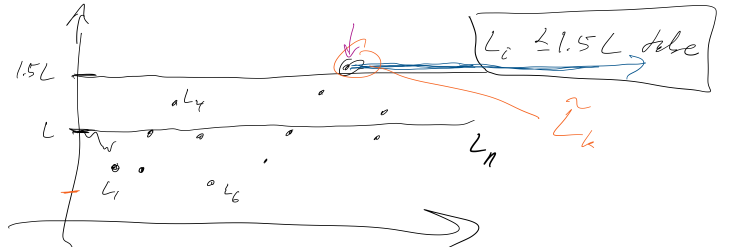
\includegraphics[width=1
  \textwidth]{fig/lec9_stoppedmartingale.png}
  \caption{Gaussian Elimination
    :
    $\vcliq{1}{\LL} = \vstar{1}{\LL} - \frac{1}{\LL(1,1)} \LL(:,1)
    \LL(:,1)^{\trp}$.}
      \label{fig:stopmart}
    \end{figure}

We state the following without proof:
\begin{claim}
\noindent
  \begin{enumerate}
  \item The sequence $\setof{\LLtil_i}$ for $i = 0, \ldots, n$ is a
    martingale.
  \item $\norm{\LL^{+/2} (\LLtil_i -  \LL) \LL^{+/2}} \leq 0.5$
    implies $\norm{\LL^{+/2} (\LL_i -  \LL) \LL^{+/2}} \leq 0.5$
  \end{enumerate}
\end{claim}
The martingale property also implies that the unconditional
expectation satisfies $\E{\LLtil_n} = \LL$.
The proof of the claim is easy to sketch: For Part 1, each difference is
zero-mean if the condition has not been violated, and is identically
zero (and hence zero-mean) if it has been violated.
For Part 2, if the martingale $\setof{\LLtil_i}$ has stopped,
then $\norm{\LL^{+/2}
  (\LLtil_i -  \LL) \LL^{+/2}} \leq 0.5$ is false, and the implication
is vacuosly true.
If the, on the other hand, if the martingale has not stopped, the
quantities are equal, because $\LLtil_i  = \LL_i$, and again it's easy
to see the implication holds.

Thus, ultimately, our strategy is goin to be to show that
$\norm{\LL^{+/2} (\LLtil_i -  \LL) \LL^{+/2}} \leq 0.5$
with high probability.
Expressed using the normalizing map $\Phi(\cdot)$,
our goal is to show that with high probability
\[
  \norm{\Phi(\LLtil_n -  \LL)} \leq 0.5.
\]

\paragraph{Stopped martingale difference sequence.}
In order to prove the spectral norm bound, we want to express the
$\setof{\LLtil_i}$ martingale in terms of a sequence of martingale
differences.
To this end, we define
$\XXtil_i = \Phi(\LLtil_i -  \LLtil_{i-1})$.
This ensures that
\begin{equation}
  \label{eq:stoppedmartingale}
  \XXtil_i
  =
  \begin{cases}
    \XX_i& \text{ if for all } j < i \text{ we have }
       \LL_i \preceq 1.5 \LL
       \\
    \matzero & \text{ otherwise }
  \end{cases}
\end{equation}
Whenever the modified martingale $\XXtil_i$ has not yet stopped, we
also introduce individual modified edge samples $\XXtil_{i,e} =
\XX_{i,e}$.
If the martingale \emph{has} stopped, i.e. $\XXtil_i = \matzero$,
then we can take these edge samples $\XXtil_{i,e}$
to be zero.
We can now write
\[
  \Phi\left(  \LLtil_n -\LL \right)
  =
    \sum_{i=1}^n \Phi(\LLtil_i - \LLtil_{i-1})
  =
  \sum_{i=1}^n \XXtil_i
  =
  \sum_{i=1}^n \sum_{e \in
    \vstar{\pi(i)}{\SS_{i-1}}}\XXtil_{i,e}
  .
\]
Thus, we can see that Equation~\eqref{eq:spectralnormgoal} is implied by
\begin{equation}
  \label{eq:zeromeanspectralnormgoal}
  \norm{\sum_{i=1}^n \XXtil_i} \leq 0.5.
\end{equation}

\subsection{Sample Norm Control}
In this Subsection, we're going to see that the norms of each
multi-edge sample is controlled throughout the algorithm.
\begin{lemma}\label{lem:cliquesample_bounded_norm}
  Given two Laplacians $\LL$ and $\SS$ on the same vertex
  set.\footnote{$\LL$ can be regarded as the original Laplacian we
    care about, while $\SS$ can be regarded as some intermediate
    Laplacian appearing during Approximate Gaussian Elimination.} If
  each multiedge $e$ of $\vstar{v}{\SS}$ has bounded norm in the following sense,
  \[ \norm{\LL^{\pinv/2}\ww_{\SS}(e)\bb_e\bb_e^{\trp}\LL^{\pinv/2}} \leq R, \]
  then each possible sampled multiedge $e'$ of $\vcliqsp{v}{\SS}$ also satisfies
  \[ \norm{\LL^{\pinv/2}\ww_{\mathrm{new}}(e')\bb_{e'}\bb_{e'}^{\trp}\LL^{\pinv/2}} \leq R. \]
\end{lemma}
\begin{proof}
  Let $\ww=\ww_{\SS}$ for simplicity. Consider a sampled edge between $i$ and $j$ with weight $\ww_{\mathrm{new}}(i,j) = \ww(i,v)\ww(j,v)/(\ww(i,v)+\ww(j,v))$.
  \begin{align*}
    \norm{\LL^{\pinv/2} \ww_{\mathrm{new}}(i,j) \bb_{ij}\bb_{ij}^{\trp}\LL^{\pinv/2}}
    &= \ww_{\mathrm{new}}(i,j) \norm{\LL^{\pinv/2} \bb_{ij}\bb_{ij}^{\trp}\LL^{\pinv/2}} \\
    &= \ww_{\mathrm{new}}(i,j) \norm{ \LL^{\pinv/2}\bb_{ij} }^2 \\
    &\leq \ww_{\mathrm{new}}(i,j) \left( \norm{\LL^{\pinv/2}\bb_{iv}}^2 + \norm{\LL^{\pinv/2}\bb_{jv}}^2 \right) \\
    &= \frac{\ww(j,v)}{\ww(i,v)+\ww(j,v)} \norm{\LL^{\pinv/2} \ww(i,v)\bb_{iv}\bb_{iv}^{\trp}\LL^{\pinv/2}} + \\
    & ~\quad \frac{\ww(i,v)}{\ww(i,v)+\ww(j,v)} \norm{\LL^{\pinv/2} \ww(j,v)\bb_{jv}\bb_{jv}^{\trp}\LL^{\pinv/2}} \\
    &\leq \frac{\ww(j,v)}{\ww(i,v)+\ww(j,v)} R + \frac{\ww(i,v)}{\ww(i,v)+\ww(j,v)} R \\
    &= R
  \end{align*}
  The first inequality uses the triangle inequality of effective resistance in $\LL$, in that effective resistance is a distance as proved in lecture 6. The second inequality just uses the conditions of this lemma.
\end{proof}
\begin{remark}
  Lemma \ref{lem:cliquesample_bounded_norm} only requires that each single multiedge has small norm instead of that the sum of all edges between a pair of vertices have small norm. And this lemma tells us, after sampling, each multiedge in the new graph still satisfies the bounded norm condition.
\end{remark}
From the Lemma, we can conclude that each edge sample $\YY_{\pi(i),e}$
satisfies
$\norm{\Phi(\YY_{\pi(i),e})} \leq R$
provided the assumptions of the
Lemma hold. Let's record this observation as a Lemma.
\begin{lemma}
  If for all $e \in \vstar{v}{\SS_i}$,
  \[
    \norm{\Phi(\ww_{\SS_i }(e)\bb_{e} \bb_{e}^{\trp})}
    \leq
    R
    .
  \]
  then all $e \in \vstar{\pi(i)}{\SS_i}$,
  \[
    \norm{\Phi(\YY_{\pi(i),e})} \leq R
 .
  \]
\end{lemma}

\paragraph{Preprocessing by multi-edge splitting.}
In the original graph of Laplacian $\LL$ of graph $G = (V,E,\ww)$, we
have for each edge $\hat{e}$ that
\[
  \ww(\hat{e}) \bb_{\hat{e}}\bb_{\hat{e}}^{\trp} \preceq \sum_e \ww(e) \bb_{e}\bb_{e}^{\trp}= \LL
\]
This also implies that
\[
  \norm{\LL^{\pinv/2}  \ww(\hat{e})  \bb_{\hat{e}}\bb_{\hat{e}}^{\trp} \LL^{\pinv/2} }\leq 1.
\]
Now, that means that if we split every original edge $e$ of the graph
into $K$ multi-edges $e_1, \ldots e_K$, with a fraction $1/K$ of the
weight, we get a new graph $G' = (V, E', \ww')$ such that
\begin{claim}
  \label{clm:edgesplit}
  \noindent
  \begin{enumerate}
  \item $G'$ and $G$ have the same graph Laplacian.
  \item $\abs{E'} = K\abs{E}$
  \item For every multi-edge in $G'$
    \[
      \norm{\LL^{\pinv/2} \ww'(e) \bb_{e}\bb_{e}^{\trp} \LL^{\pinv/2}
      }\leq 1/K.
    \]
  \end{enumerate}
\end{claim}
Before we run Approximate Gaussian Elimination, we are going to do
this multi-edge splitting to ensure we have control over multi-edge
sample norms.
%
Combined with Lemma~\ref{lem:cliquesample_bounded_norm} immediately
establishes the next lemma, because we start off with all multi-edges
having bounded norm and only produce multi-edges with bounded norm.
\begin{lemma}
  \label{lem:edgesampnorm}
  When Algorithm~\ref{alg:apxge} is run on the (multi-edge) Laplacian of $G'$,
  arising from splitting edges of $G$ into $K$ multi-edges, the every
  edge sample $\YY_{\pi(i),e}$ satisfies
  \[
    \norm{\Phi(\YY_{\pi(i),e})} \leq 1/K
 .
  \]
\end{lemma}
As we will see later $K = 200 \log^2 n$ suffices.

\subsection{Random Matrix Concentration from Trace Exponentials}
Let us recall how matrix-valued variances come into the picture when
proving concentration following the strategy from Matrix Bernstein in
Lecture 8.

For some matrix-valued random variable $\XX \in \symsetn$,
we'd like to show $\Pr[ \norm{\XX} \leq 0.5 ]$.
Using Markov's inequality, and some observations about matrix
exponentials and traces, we saw that for all $\theta > 0$,
\begin{equation}
  \label{eq:masterprob}
  \Pr[ \norm{\XX} \geq 0.5 ]
  \leq
  \exp(-0.5\theta ) \left(\E{\trace{ \exp\left(\theta \XX\right)}}
  +
  \E{\trace{ \exp\left(-\theta \XX\right)}}
  \right)
  .
\end{equation}
We then want to bound $\E{\trace{ \exp\left(\theta \XX\right)}}$
using Lieb's theorem.
We can handle $\E{\trace{ \exp\left(-\theta \XX\right)}}$ similarly.
\begin{theorem}[Lieb]
  \label{thm:Lieb}
  Let $f:S^n_{++}\to\R$ be a matrix function given by
  \[ f(\AA) = \trace{\exp\left(\HH+\log(\AA)\right)} \]
  for some $\HH\in S^n$. Then $-f$ is convex (i.e. $f$ is concave).
\end{theorem}
As observed by Tropp, this is useful for proving matrix concentration statements.
Combined with Jensen's inequality, it gives that for a random matrix
$\XX \in \symsetn $ and a fixed $\HH \in \symsetn$
\[
  \E{\trace{ \exp\left(\HH+\XX\right)}}
    \leq
    \trace{ \exp\left(\HH+\log(\E{\exp(\XX)})\right)}
  .
\]
The next crucial step was to show that it suffices to obtain an upper
bound on the matrix $\E{\exp(\XX)}$ w.r.t the Loewner order.
Using the following three lemmas, this conclusion is an immediate
corollary.
\begin{lemma}\label{lem:trexpmono}
  If $\AA\preceq\BB$, then $\trace{\exp(\AA)}\leq\trace{\exp(\BB)}$.
  % i.e. $\ZZ \mapsto \trace{\exp(\ZZ)}$ is monotone increasing.
\end{lemma}
\begin{lemma}\label{lem:logmono}
  If $0\prec\AA\preceq\BB$, then $\log(\AA)\preceq\log(\BB)$.
\end{lemma}
\begin{lemma}\label{lem:ineq_log}
  $\log(\II+\AA) \preceq \AA$ for $\AA\succ-\II$.
\end{lemma}
%
\begin{corollary}
  \label{cor:trexpub}
  For a random matrix
  $\XX \in \symsetn $ and a fixed $\HH \in \symsetn$,
  if $\E{\exp(\XX)} \preceq \II + \UU$ where $\UU \succ -\II$, then
\[
  \E{\trace{ \exp\left(\HH+\XX\right)}}
    \leq
    \trace{ \exp\left(\HH+\UU\right)}
  .
\]
\end{corollary}

% \begin{corollary}\label{cor:trexpmono}
%   If $\AA\preceq\BB$, then $\trace{\exp(\AA)}\leq\trace{\exp(\BB)}$,
%   i.e. $\XX \mapsto \trace{\exp(\XX)}$ is monotone increasing.
% \end{corollary}
% \begin{lemma}\label{lem:logmono}
%   If $0\prec\AA\preceq\BB$, then $\log(\AA)\preceq\log(\BB)$.
% \end{lemma}

\subsection{Mean-Exponential Bounds from Variance Bounds}
To use Corollary~\ref{cor:trexpub}, we need to construct useful upper
bounds on $\E{\exp(\XX)}$.
This can be done, starting from the following lemma.
\begin{lemma}\label{lem:ineq_exp}
  $\exp(\AA) \preceq \II + \AA + \AA^2$ for $\|\AA\|\leq1$.
\end{lemma}
If $\XX$ is zero-mean and $\norm{\XX} \leq 1$,
this means that $\E{\exp(\XX)} \preceq \II + \E{\XX^2}$,
which is how we end up wanting to bound the matrix-valued variance $\E{\XX^2}$.
In the rest of this Subsection, we're going to see the matrix-valued variance of the stopped
martingale is bounded throughout the algorithm.

Firstly, we note that for a single edge sample $\XXtil_{i,e}$,
by Lemma~\ref{lem:edgesampnorm}, we have that
\[
  \norm{\XXtil_{i,e}} \leq
  \norm{\Phi\left( \YY_{\pi(i),e} - \E{\YY_{\pi(i),e}} \right)}
    \leq 1/K,
\]
using that $\norm{\AA-\BB} \leq \max( \norm{\AA}, \norm{\BB} )$, for
$\AA, \BB \succeq \matzero$, and $\norm{\E{\AA}} \leq \E{\norm{\AA}}$
by Jensen's inequality.

Thus, if $0 < \theta \leq K$, we have that
\begin{align}
  \label{eq:edgelogexp}
  \E{ \exp(\theta \XXtil_{i,e}) \mid \text{preceding samples} }
  &\preceq
      \II +
    \E{(\theta \XXtil_{i,e})^2 \mid \text{preceding samples} }
  \\ \nonumber   &\preceq
        \II +
    \frac{1}{K}\theta^2\cdot
    \E{\Phi(\YY_{\pi(i),e}) \mid \text{preceding samples} }
\end{align}
% \begin{lemma}
%   \label{lem:edgelogexp}
%   \[
%     \log \Ex{\XX_{v_i,d_i-1}}\exp(\theta\XX_{v_i,d_i}) \preceq
%     \theta^2 R \cdot
%     \Ex{\XX_{v_i,d_i-1}}\Phi(\YY_{v_i,d_i})
%   \]
% \end{lemma}



\subsection{The Overall Mean-Trace-Exponential Bound}

We will use $\Ex{(<i)} $ to denote expectation over variables preceding the
$i$th elimination step.
We are going to refrain from explicitly writing out conditioning in
our expectations, but any \emph{inner} expectation that appears inside another
\emph{outer} expectation should be taken as conditional on the outer
expectation.
We are going to use $d_i$ to denote the multi-edge degree of vertex
$\pi(i)$ in $\SS_{i-1}$. This is exactly the number of edge samples in
the $i$th elimination.
Note that there is no elimination at step $n$ (the algorithm is
already finished). As a notational convenience, let's write $\hat{n} =
n-1$.
With all that in mind, we bound the mean-trace-exponential for some
parameter
$0 <\theta \leq 0.5/\sqrt{K}$
\begin{align}
    \label{eq:fulltrexpub1}
&  \Ex{}\trace{\exp(\theta\sum_{i = 1}^{\hat{n}}\XXtil_{i} )}
  \\ \nonumber
&  = \Ex{(<\hat{n})} \Ex{\pi(\hat{n})} \Ex{\XXtil_{\hat{n},1}} \cdots \Ex{\XXtil_{\hat{n},d_{\hat{n}}-1}}  \Ex{\XXtil_{\hat{n},d_{\hat{n}}}}
   \tr\exp\left( \underbrace{\sum_{i = 1}^{\hat{n}-1}\theta\XXtil_{i}
     + \sum_{e =1}^{d_{\hat{n}}-1}\theta\XXtil_{\hat{n},e}}_{\HH}
    +\theta \XXtil_{\hat{n},d_{\hat{n}}} \right)
   \tag*{$\XXtil_{\hat{n},1} \ldots, \XXtil_{\hat{n},d_{\hat{n}}}$  are independent
    conditional on $(<\hat{n}), \pi(\hat{n})$
  }
\\  \nonumber
&  \leq \Ex{(<\hat{n})} \Ex{\pi(\hat{n})} \Ex{\XXtil_{\hat{n},1}} \cdots \Ex{\XXtil_{\hat{n},d_{\hat{n}}-1}}
   \tr\exp\left(\sum_{i = 1}^{\hat{n}-1}\theta\XXtil_{i}
     +  \sum_{e =1}^{d_{\hat{n}}-1}\theta\XXtil_{\hat{n},e}
    +  \frac{1}{K}\theta^2\cdot
    \Ex{\XXtil_{\hat{n},d_{\hat{n}}}}{\Phi(\YY_{\pi(\hat{n}), d_{\hat{n}}})}
  \right)
  \tag*{By Equation~\eqref{eq:edgelogexp} and Corollary~\ref{cor:trexpub}
  .
  }
  \\ \nonumber
&  \vdots
 \tag*{ Repeat for each multi-edge sample $\XXtil_{\hat{n},1} \ldots,
       \XXtil_{\hat{n},d_{\hat{n}}-1}$ }
\\  \nonumber
&  \leq  \Ex{(<\hat{n})} \Ex{\pi(\hat{n})}
   \tr\exp\left(\sum_{i = 1}^{\hat{n}-1}\theta\XXtil_{i}
     +  \sum_{e =1}^{d_{\hat{n}} }
     \frac{1}{K}\theta^2\cdot
    \Ex{\XXtil_{\hat{n},e}}{\Phi(\YY_{\pi(\hat{n}), e})}
     \right)
 \\  \nonumber
&  = \Ex{(<\hat{n})} \Ex{\pi(\hat{n})}
   \tr\exp\left(\sum_{i = 1}^{\hat{n}-1}\theta\XXtil_{i}
     +
     \frac{1}{K}\theta^2\vcliq{\pi(\hat{n})}{\SS_{\hat{n}-1}}
  \right)
\end{align}
To further bound the this quantity, we now need to deal with the
random choice of $\pi(\hat{n})$.
We'll be able to use this to bound the trace-exponential in a very
strong way.
From a random matrix perspective, it's the following few
steps that give the analysis it's surprising strength.

We can treat
$\frac{1}{K}\theta^2\vcliq{\pi(\hat{n})}{\SS_{\hat{n}-1}}$ as a random
matrix.
It is not zero-mean, but we can still bound the trace-exponential
using Corollary~\ref{cor:trexpub}.

We can also bound the expected matrix exponential in
that case, using a simple corollary of Lemma~\ref{lem:ineq_exp}.
\begin{corollary}\label{cor:ineq_exp_cher}
  $\exp(\AA) \preceq \II + (1+R)\AA $
  for $\matzero \preceq \AA$ with $\norm{\AA} \leq R$.
\end{corollary}
\begin{proof}
  The conclusion follows after observing that for $\matzero \preceq \AA$ with $\norm{\AA} \leq R$,
  we have $\AA^2 \preceq R \AA$.
  We can see this by considering the spectral decomposition of $\AA$
  and dealing with each eigenvalue separately.
\end{proof}

Next, we need a simple structural observation about the cliques
created by elimination:
\begin{claim}
  \label{clm:cliquevsstar}
  \[
    \vcliq{\pi(i)}{\SS_i} \preceq \vstar{\pi(i)}{\SS_i} \preceq \SS_i
  \]
\end{claim}
\begin{proof}
  The first inequality is immediate from
  $
     \vcliq{\pi(i)}{\SS_i} \preceq   \vcliq{\pi(i)}{\SS_i} + \ll_i\ll_i^\trp
     =
     \vstar{\pi(i)}{\SS_i}
   $
   .
   The latter inequality $\vstar{\pi(i)}{\SS_i} \preceq \SS_i$
  follows from the star being a subgraph of the whole Laplacian $\SS_i$.
\end{proof}

Next we make use of the fact that $\XXtil_{i}$ is from the
difference sequence of the \emph{stopped} martingale.
This means we can assume
\[
  \SS_{i} \preceq 1.5 \LL,
\]
since
otherwise $\XXtil_{i} = \matzero$ and we get an even better
bound on the trace-exponential.
To make this formal, in Equation~\eqref{eq:fulltrexpub1},
we ought to do a case analysis that also includes
the case $\XXtil_{i} = \matzero$ when the martingale has
stopped, but we omit this.

Thus we can conclude by Claim~\ref{clm:cliquevsstar} that
\[
  \norm{\Phi(\vcliq{\pi(i)}{\SS_{i}})} \leq 1.5.
\]

By our assumption $0 <\theta \leq 0.5/\sqrt{K}$, we have
$\norm{\frac{1}{K}\theta^2\Phi(\vcliq{\pi(i)}{\SS_{i-1}})}
\leq 1$, so that by Corollary~\ref{cor:ineq_exp_cher},
\begin{align}
  \Ex{\pi(i)}
  \exp\left(\
     \frac{1}{K}\theta^2\Phi(\vcliq{\pi(i)}{\SS_{i-1}})
  \right)
  &\preceq
  \II
  +
  \frac{2}{K} \theta^2\Ex{\pi(i)}
    \Phi(\vcliq{\pi(i)}{\SS_{i-1}})
  \\
  &\preceq
  \II
  +
  \frac{2}{K} \theta^2\Ex{\pi(i)}
  \Phi(\vstar{\pi(i)}{\SS_{i-1}})
  \tag*{by Claim~\ref{clm:cliquevsstar}.}
\end{align}
Next we observe that, because every multi-edge appears in exactly two
stars, and $\pi(i)$ is chosen uniformly at random among the $n+1-i$
vertices that $\SS_{i-1}$ is supported on, we have
\[
  \Ex{\pi(i)}
  \vstar{\pi(i)}{\SS_{i-1}}
  =
  2\frac{1}{n+1-i}\SS_{i-1}
  .
\]
And, since we assume $\SS_{i} \preceq 1.5 \LL$, we further get
\[
  \Ex{\pi(i)}
  \exp\left(\
     \frac{1}{K}\theta^2\Phi(\vcliq{\pi(i)}{\SS_{i-1}})
  \right)
  \preceq
  \II
  +
  \frac{6\theta^2}{K(n+1-i)}\II
  .
\]
We can combine this with Equation~\eqref{eq:fulltrexpub1} and
Corollary~\ref{cor:trexpub} to get
\begin{align*}
  &  \Ex{}\trace{\exp(\theta\sum_{i = 1}^{\hat{n}}\XXtil_{i} )}
     \\*  \nonumber
  &  \leq
    \Ex{(<\hat{n})} \Ex{\pi(\hat{n})}
   \tr\exp\left(\sum_{i = 1}^{\hat{n}-1}\theta\XXtil_{i}
     +
     \frac{1}{K}\theta^2\vcliq{\pi(\hat{n})}{\SS_{\hat{n}-1}}
    \right)
\\  \nonumber
  &  \leq
    \Ex{(<\hat{n})}
   \tr\exp\left(\sum_{i = 1}^{\hat{n}-1}\theta\XXtil_{i}
     +
    \frac{6\theta^2}{K(n+1-i)}\II
  \right)
\end{align*}
And by repeating this analysis for each term $\XXtil_{i}$, we get
\begin{align*}
 \Ex{}\trace{\exp(\theta\sum_{i = 1}^{\hat{n}}\XXtil_{i} )}
&\leq
   \tr\exp\left(\sum_{i = 1}^{\hat{n}}
    \frac{6\theta^2}{K(n+1-i)}\II
    \right)
\\
  &\leq
\tr\exp\left(
    \frac{7\theta^2\log(n)}{K}\II
    \right)
\\
  &=
    n\exp\left(
    \frac{7\theta^2\log(n)}{K}
    \right)
\end{align*}
Then, by choosing $K = 200 \log^2 n$ and $\theta = 0.5 \sqrt{K}$,
we get
\[
\exp(-0.5 \theta ) \Ex{}\trace{\exp(\theta\sum_{i =
    1}^{\hat{n}}\XXtil_{i} )}
\leq
\exp(-0.5 \theta )
 n\exp\left(
    \frac{7\theta^2\log(n)}{K}
  \right)
  \leq
  1/n^5.
\]
$\Ex{}\trace{\exp(-\theta\sum_{i =
    1}^{\hat{n}}\XXtil_{i} )}$ can be bounded by an identical
argument, so that Equation~\eqref{eq:masterprob} gives
\[
  \Pr\left[ \norm{
\sum_{i =
    1}^{\hat{n}}\XXtil_{i}
  } \geq 0.5 \right] \leq 2/n^5.
  \]
Thus we have established $\norm{
\sum_{i =
    1}^{\hat{n}}\XXtil_{i}
  } \leq 0.5 $ with high probability
  (Equation~\eqref{eq:zeromeanspectralnormgoal}), and this in turn
  implies Equation~\eqref{eq:spectralnormgoal}, and finally
  Equation~\eqref{eq:relerrgoal}:
  \[
0.5 \LL
\preceq
\matlow \matlow^{\trp}
\preceq 1.5 \LL
.
\]

Now, all that's left to note is that the running time is linear in the
multi-edge degree of the vertex being eliminated in each iteration (and
this also bounds the number of non-zero entries being created in
$\matlow$).
The total number of multi-edges left in the remaining graph stays
constant at $K m = O(m\log^2 n)$.
Thus the expected degree in the $i$th elimination is $K m/(n+i-1)$,
because the remaining number of vertices is $n+i-1$.
Hence the total running time and total number of non-zero entries
created can both be bounded as
\[
  Km\sum_i 1/(n+i-1) = O(m\log^3 n)
  .
  \]
We can further prove that the bound $O(m\log^3 n)$ on running time and
number of non-zeros in $\LL$ holds with high probability
(e.g. $1-1/n^5$).
To show this, we essentially need a scalar Chernoff bound, in except
the degrees are in fact not independent, and so we need a scalar
martingale concentration result, e.g. Azuma's Inequality.
This way, we complete the proof of Theorem~\ref{thm:apxgauss}.
\FloatBarrier

% \todo{reenable lecture}
%\bibliographystyle{alpha}
%\bibliography{refs}


%%% Local Variables:
%%% mode: latex
%%% TeX-master: "agao21_script"
%%% TeX-engine: luatex
%%% End: